\documentclass[12pt,letterpaper]{article}
\usepackage[utf8]{inputenc}
\usepackage[spanish]{babel}
\usepackage{graphicx}
\usepackage[left=2cm,right=2cm,top=2cm,bottom=2cm]{geometry}
\usepackage{graphicx} % figuras
% \usepackage{subfigure} % subfiguras
\usepackage{float} % para usar [H]
\usepackage{amsmath}
%\usepackage{txfonts}
\usepackage{stackrel} 
\usepackage{multirow}
\usepackage{enumerate} % enumerados
\renewcommand{\labelitemi}{$-$}
\renewcommand{\labelitemii}{$\cdot$}
% \author{}
% \title{Caratula}
\begin{document}

% Fancy Header and Footer
% \usepackage{fancyhdr}
% \pagestyle{fancy}
% \cfoot{}
% \rfoot{\thepage}
%

% \usepackage[hidelinks]{hyperref} % CREA HYPERVINCULOS EN INDICE

% \author{}
\title{Caratula}

\begin{titlepage}
\begin{center}
\large{UNIVERSIDAD PRIVADA-DE-TACNA}\\
\vspace*{-0.025in}
\begin{figure}[htb]
\begin{center}

\includegraphics[width=8cm]{./Imagenes/logo}
\end{center}
\end{figure}
\vspace*{0.15in}
INGENIERIA DE SISTEMAS  \\

\vspace*{0.5in}
\begin{large}
TITULO:\\
\end{large}

\vspace*{0.1in}
\begin{Large}
\textbf{Laboratorio No 02} \\
\end{Large}

\vspace*{0.3in}
\begin{Large}
\textbf{CURSO:} \\
\end{Large}

\vspace*{0.1in}
\begin{large}
BASE DE DATOS II\\
\end{large}

\vspace*{0.3in}
\begin{Large}
\textbf{DOCENTE(ING):} \\
\end{Large}

\vspace*{0.1in}
\begin{large}
 Patrick Cuadros Quiroga\\
\end{large}

\vspace*{0.2in}
\vspace*{0.1in}
\begin{large}
Integrantes: \\
\begin{flushleft}
J		\hfill	(201) \\
David Damian Mamani 		                  \hfill	 (2016055194) \\
Andre Sebastian Reinoso Aranda          	\hfill	(2016055275) \\
M      	\hfill	(201) \\

\end{flushleft}
\end{large}
\end{center}

\end{titlepage}


\tableofcontents % INDICE
\thispagestyle{empty} % INDICE SIN NUMERO
\newpage
\setcounter{page}{1} % REINICIAR CONTADOR DE PAGINAS DESPUES DEL INDICE


\section{Desarrollo} 
Ejercicio 1: Obtener al estudiante con el ID Uno
\begin{itemize}
	\item Codigo
	\\Mediante el código se podrá buscar en la base de datos (Tabla Estudiante) al estudiante siempre y cuando su nombre sea “Bill”
	\begin{center}
	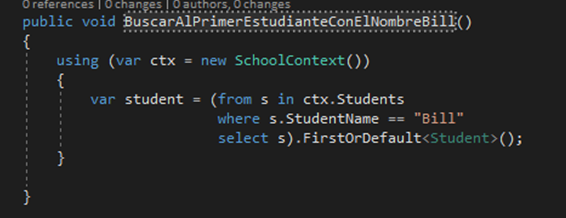
\includegraphics[width=15cm]{./Imagenes/1a} 
	\end{center}
	\item Gestor de base de Datos
	\\Esta sentencia que es generada por el código en el gestor de la base de datos muestra como efectúa la selección del código en la base de datos el cual nos mostrara el estudiante con el nombre “Bill”
	\begin{center}
	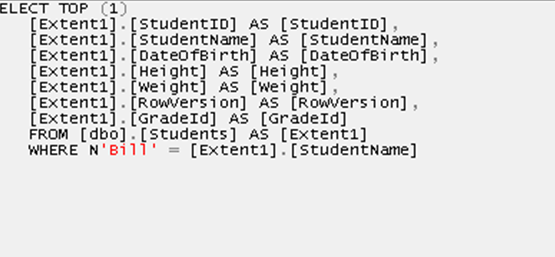
\includegraphics[width=15cm]{./Imagenes/1b} 
	\end{center}
\end{itemize} 

\newpage
Ejercicio 2: Buscar Estudiantes Agrupados Por Grado

\begin{itemize}
	\item Codigo
	\\Consiste en que el código buscara al estudiante dependiendo al grado, es decir que  evaluara a cada estudiante con los datos ingresados en la tabla grade
	\begin{center}
	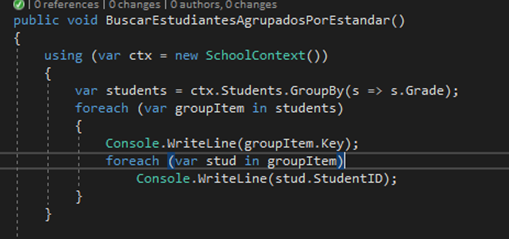
\includegraphics[width=15cm]{./Imagenes/2a} 
	\end{center}
	
	\item Gestor de base de Datos
	\\La sentencia generada seleccionara la tabla “Grade” y la tabla “Student”, seguidamente tomara una variable “Distinct1” el cual tomara los valores de la tabla “Grade” y por otro lado la variable “Extent3” tomara los valores de la tabla “Student”, Después lo evaluara para mostrar los valores correspondientes.
	\\
\begin{center}
	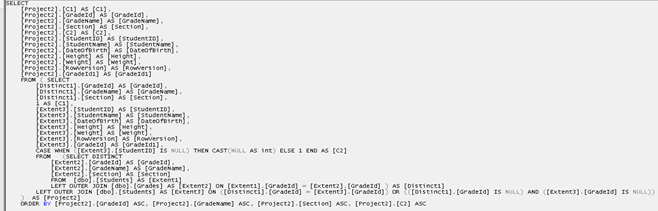
\includegraphics[width=15cm]{./Imagenes/2b} 
	\end{center}
	
\end{itemize} 
\newpage

Ejercicio 3: Obtener listado de estudiantes ordenados por nombre

\begin{itemize}
	\item Codigo
	\\El siguiente código ordenara la tabla “Student” por dependiendo del nombre, es decir, que seguirá el orden alfabético.

	\begin{center}
	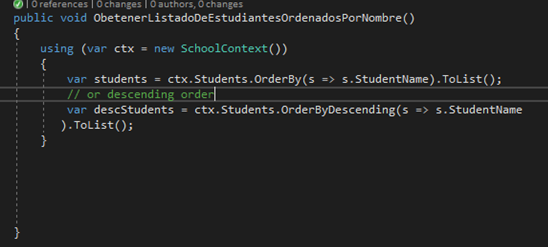
\includegraphics[width=15cm]{./Imagenes/3a} 
	\end{center}

	\item Gestor de base de Datos 
	\\La sentencia tomará los valores de la tabla estudiante en “Extent1” de tal modo ordenada la posición de ella mediante el “Order By” que estará sujeto a “StudentName” con la propiedad  
	\begin{center}
	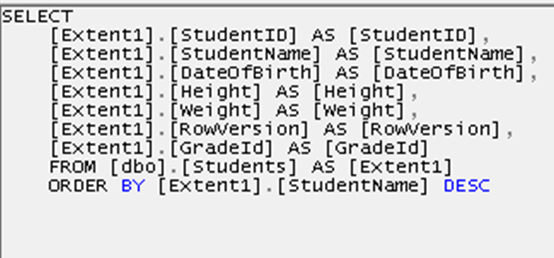
\includegraphics[width=15cm]{./Imagenes/3b} 
	\end{center}
	
\end{itemize} 
\newpage
Ejercicio 4: Insertar estudiantes satisfactoriamente

\begin{itemize}
	\item Codigo
	\\Consiste en que el código buscara al estudiante dependiendo al grado, es decir que  
evaluara a cada estudiante con los datos ingresados en la tabla "Grade"

	\begin{center}
	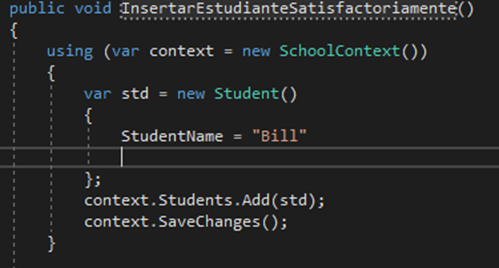
\includegraphics[width=15cm]{./Imagenes/4a} 
	\end{center}

	\item Gestor de base de Datos 
	\\La sentencia generada seleccionara la tabla “Grade” y la tabla “Student”, seguidamente tomara una variable “Distinct1” el cual tomara los valores de la tabla “Grade” y por otro lado la variable “Extent3” tomara los valores de la tabla “Student”, Después lo evaluara para mostrar los valores correspondientes. 
	\begin{center}
	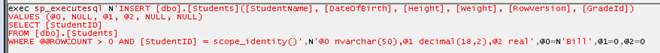
\includegraphics[width=15cm]{./Imagenes/4b} 
	\end{center}
	
\end{itemize} 
\newpage
Ejercicio 5: Eliminar El Primer Grade Satisfactoriamente

\begin{itemize}
	\item Codigo
	\\En el siguiente código Eliminara al primero estudiante.

	\begin{center}
	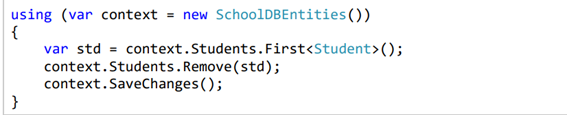
\includegraphics[width=15cm]{./Imagenes/5a} 
	\end{center}

	\item Gestor de base de Datos 
	\\En la sentencia seleccionar la tabla “Student”, seguidamente eliminará el Student con el código correspondiente que en este caso será “1”
	\begin{center}
	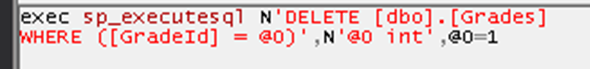
\includegraphics[width=15cm]{./Imagenes/5b} 
	\end{center}
	
\end{itemize} 
\newpage
Ejercicio 6: Agregar Tres Grades Satisfactoriamente

\begin{itemize}
	\item Codigo
	\\El siguiente código evaluara la lista “Grades” de tal modo que insertara nuevos parámetros o valores a la lista. Seguidamente agregara los datos y guardara cambios

	\begin{center}
	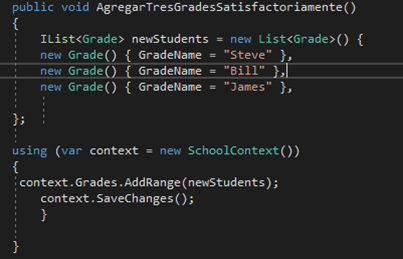
\includegraphics[width=15cm]{./Imagenes/6a} 
	\end{center}

	\item Gestor de base de Datos 
	\\La sentencia insertara los parámetros establecidos en el código, de tal como que seleccionara la tabla correspondiente e insertara los datos.
	\begin{center}
	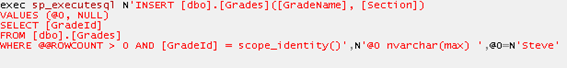
\includegraphics[width=15cm]{./Imagenes/6b} 
	\end{center}
\begin{center}
	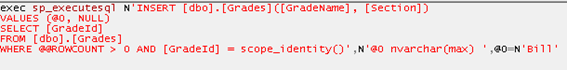
\includegraphics[width=15cm]{./Imagenes/6c} 
	\end{center}
\begin{center}
	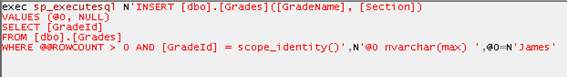
\includegraphics[width=15cm]{./Imagenes/6d} 
	\end{center}
	
\end{itemize} 

\end{document}
